%!TEX TS-program = xelatex
%!TEX encoding = UTF-8 Unicode

%%%  Syllabus template for use with style files at http://kjhealy.github.com/latex-custom-kjh
%%%  Kieran Healy

\documentclass[11pt,article,oneside]{memoir}

% packages
\usepackage{org-preamble-xelatex} 

\AtBeginBibliography{\small}

% Definitions
\def\myauthor{Author}
\def\mytitle{Title}
\def\mycopyright{\myauthor}
\def\mykeywords{}
\def\mybibliostyle{plain}
\def\mybibliocommand{}
\def\mysubtitle{}
\def\myaffiliation{Louisiana State University}
\def\myaddress{100 Design}
\def\myemail{harmon1@lsu.edu}
\def\myweb{https://baharmon.github.io/}
\def\myphone{919.622.8414}
\def\myversion{}
\def\myrevision{}
\def\myaffiliation{\ \\Louisiana State University}
\def\myauthor{Brendan Harmon}
\def\mykeywords{Landscape Architecture, Syllabus, Graduate}
\def\mysubtitle{Syllabus}
\def\mytitle{{\normalsize \textsc{LA} 3001\newline} \huge \bfseries Landscape Planning Studio}

\begin{document}

\setlength\bibitemsep{0.75em}

% fonts
\defaultfontfeatures{}
\defaultfontfeatures{Scale=MatchLowercase}         
\setmainfont[Scale=1, Path = fonts/lato/,BoldItalicFont=Lato-RegIta,BoldFont=Lato-Reg,ItalicFont=Lato-LigIta]{Lato-Lig}
\setsansfont[Scale=1, Path = fonts/lato/,BoldItalicFont=Lato-RegIta,BoldFont=Lato-Reg,ItalicFont=Lato-LigIta]{Lato-Lig}
\setmonofont[Mapping=tex-text,Scale=0.8,Path = fonts/inconsolata/]{i}

\def\ind{\hangindent=1 true cm\hangafter=1 \noindent}
\def\labelitemi{$\cdot$}
\chapterstyle{article-4-sans}  
\title{\LARGE \mytitle}     
\author{\Large\myauthor \newline \footnotesize\texttt{\noindent\myemail}}
\date{Fall 2017. Design 217.\newline Tuesday \& Thursday 1:30am--5:20pm.}
\published{\,}

\maketitle

% -------------------------------- COVER PAGE -------------------------------- 

% full page image with no borders, 30% opacity, greyscale
% image: orthoimagery | flooded elevation 

% -------------------------------- DESCRIPTION -------------------------------- 

\section{Course Description}

%This course is an introduction to digital design for landscape architects. 
%In this course you will develop a creative digital design process 
%seamlessly integrating research and design
%using geographic information systems (GIS),
%3D modeling and rendering, and
%visual programming. 
%You will learn how to use geospatial data 
%to model and analyze landscapes
%and visual programming to 
%parametrically model and transform new landforms. 
%You will learn how to model plants -- from trees to grasses -- in 3D, 
%automatically distribute them across your digital landscape,
%and render photorealistic scenes. 
%Each week you will spend a day in a workshop
%learning new methods
%and a day developing your projects.\\

\noindent \textbf{Format}
Workshop, desk critiques, and pinup. \\

%\noindent In preparation for this course please read:
%\nocite{*} \printbibliography[keyword=intro, heading=none]

%\begin{figure}
%    \begin{center}
%        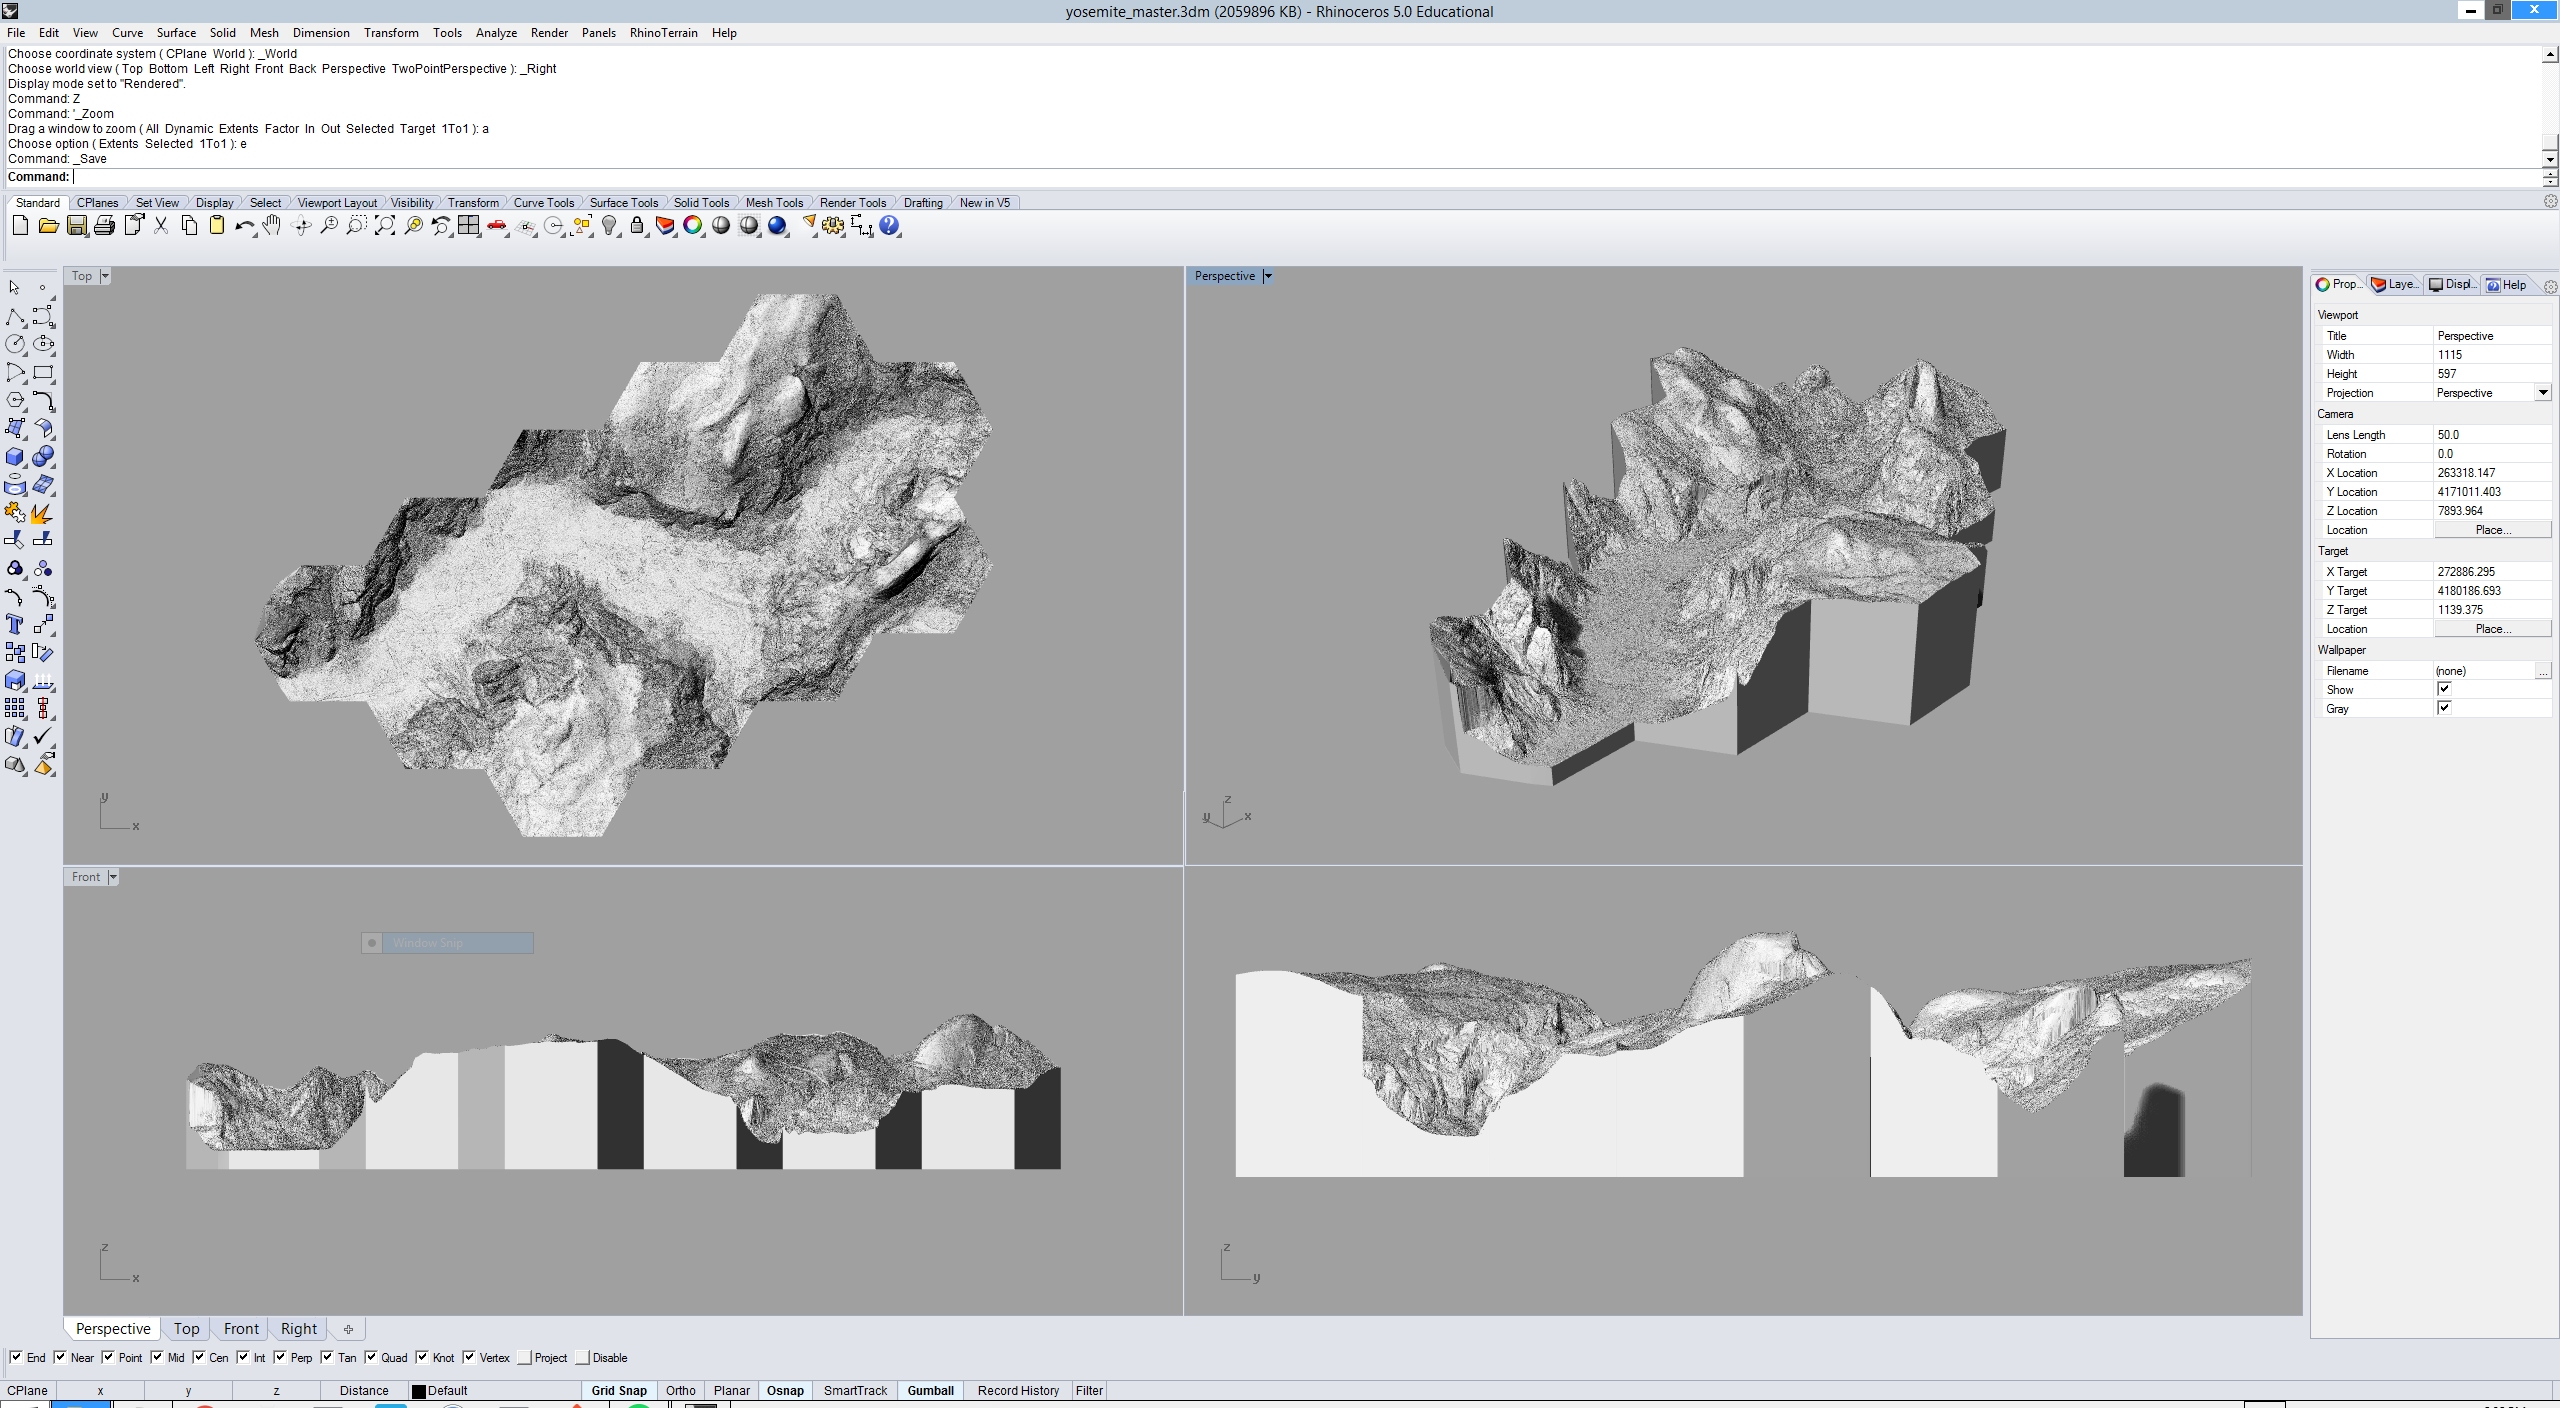
\includegraphics[width=\textwidth]{images/yosemite_1.png}
%        \caption{...}
%        \label{fig:yosemite}
%    \end{center}
%\end{figure}

\clearpage

% -------------------------------- SCHEDULE -------------------------------- 
\section{Course Schedule}

\begin{table}[H]
\small
\begin{tabular}{l l @{\hskip 1cm}l}
%
\textbf{1} & Design charrette\\
\textbf{2} & Field trip\\
\textbf{3} & Precedent studies\\
\textbf{4} & Cartography & \textbf{Site visit:} Golden Meadows\\
\textbf{5} & Topography\\
\textbf{6} & Infrastructure\\
\textbf{7} & Hydrology\\
\textbf{8} & Sediment\\
\textbf{9} & Ecosystems\\
\textbf{10} & Map production & \textbf{Mid-review}\\
\textbf{11} & Ecological baselines & \textbf{Digital fabrication workshop}\\
\textbf{12} & Suitability analysis\\
\textbf{13} & Masterplanning I\\
\textbf{14} & Masterplanning II\\
\textbf{15} & Masterplanning III & \textbf{Final review}\\\\
%
\end{tabular}
\end{table}

%\clearpage

% -------------------------------- SESSIONS -------------------------------- 
\section{Sessions}

\renewcommand*{\bibfont}{\footnotesize}

\noindent \textbf{Design charrette}
A design charrette for the Louisiana Governor's Mansion.\\

\noindent \textbf{Field trip}
We will visit Washington DC and New York City. 
In Washington DC we will explore the traces of the L'Enfant plan
and tour the museums and monuments.
In New York City we will visit design firms including 
MVVA, SCAPE, and Robert A.M. Stern Architects  
and tour projects like the Brooklyn Bridge Park and the High Line.
We will also learn about 
US Army Corps of Engineers' coastal resilience projects
and tour their projects on Long Beach Island.\\

% reading: 

%\nocite{*} \printbibliography[keyword=fabrication, heading=none]
%\vspace*{0.5em}

\noindent \textbf{Precedent studies}\\
% Presentation of precedent studies \\
%
Louisiana Coastal Masterplan | \url{http://coastal.la.gov/2017-coastal-master-plan/}\\
Netherlands National Coastal Strategy | \\
\url{http://rijksoverheid.minienm.nl/nvk/NationalCoastalStrategy.pdf}\\
The Sand Engine | \url{http://www.dezandmotor.nl/en/}\\
Delta Works | \url{http://www.deltawerken.com/}\\
% https://deltaprogramma2017.deltacommissaris.nl/
% http://rijksoverheid.minienm.nl/nvk/NationalCoastalStrategy.pdf
MOSE | \url{https://www.mosevenezia.eu/}\\
Oystertecture | \url{http://www.scapestudio.com/projects/oyster-tecture/}\\
New Meadowlands | \url{http://newmeadowlands.org/}\\
Fresh Kills | \url{http://freshkillspark.org/}\\
% Fresh Kills Competition: http://www1.nyc.gov/assets/planning/download/pdf/plans/fkl/fkl.pdf
% Fresh Kills Masterplan: http://freshkillspark.org/wp-content/uploads/2013/07/Fresh-Kills-Park-Draft-Master-Plan.pdf


\noindent \textbf{Cartography}
% Data acquisition
%
% Readings: Ganges Water Machine, Cartographic Grounds, etc
%Examples: http://atlas-for-the-end-of-the-world.com/world_maps_main.html
\\

\noindent \textbf{Site visit}
\\


\noindent \textbf{Topography}
\\

\noindent \textbf{Infrastructure}
\\

\noindent \textbf{Hydrology}
% watersheds, water accumulation, flow, flooding
\\

\noindent \textbf{Sediment}
\\

\noindent \textbf{Ecosystems}
% Image classification, habitat identification, fragmentation, diversity
\\

\noindent \textbf{Map production}
%Multi-scale maps
%Mid review
%
\\

\noindent \textbf{Mid-review}
\\

\noindent \textbf{Ecological baselines}
%Ecological baseline seminar
	%Readings: rewilding, etc
%Digital fabrication workshop
	%Resources: 
%Ecological baseline charrette
\\
%
\nocite{*} \printbibliography[keyword=baselines, heading=none]
\vspace*{0.5em}


\noindent \textbf{Digital fabrication workshop}
\\

\noindent \textbf{Suitability analysis}
...\\
%
\nocite{*} \printbibliography[keyword=suitability, heading=none]
\vspace*{0.5em}

\noindent \textbf{Masterplanning I}
\\

\noindent \textbf{Masterplanning II}
% Planting design\\
\\

\noindent \textbf{Masterplanning III}
\\

\noindent \textbf{Final review}
% deliverables: Illustrative masterplan
\\

%
%\nocite{*} \printbibliography[keyword=fabrication, heading=none]
%\vspace*{0.5em}


%\clearpage

% -------------------------------- Software -------------------------------- 
\section{Software}
GRASS GIS | \url{https://grass.osgeo.org/}\\
QGIS | \url{https://www.qgis.org/}\\
ArcGIS | \url{http://www.esri.com/arcgis/about-arcgis/}\\
Rhinoceros | \url{https://www.rhino3d.com/}\\
RhinoTerrain | \url{http://www.rhinoterrain.com/}\\
RhinoCAM | \url{https://mecsoft.com/rhinocam-software/}\\
Adobe Creative Cloud | \url{http://www.adobe.com/creativecloud.html}\\

% -------------------------------- Resources -------------------------------- 
\section{Resources}
Intro to GRASS GIS | \url{https://ncsu-geoforall-lab.github.io/grass-intro-workshop/}\\
Hydrology in GRASS GIS | \url{https://grasswiki.osgeo.org/wiki/Hydrological_Sciences}\\

\clearpage
% -------------------------------- Readings -------------------------------- 
\section{Readings}
\renewcommand*{\bibfont}{\normalsize} %\small
\vspace*{0.5cm}
\nocite{*}
\setlength\bibitemsep{1\baselineskip}
\printbibliography[heading=none]

\clearpage

% -------------------------------- Policies -------------------------------- 
\section{Policies}

\noindent \textbf{Time Commitment Expectations}
LSU's general policy states that for each credit hour, you (the student) should plan to
spend at least two hours working on course related activities outside of class. Since this course is for three credit hours, you should expect to spend a minimum of six hours outside of class each week working on assignments for this course. For more information see: 
\url{http://catalog.lsu.edu/content.php?catoid=12&navoid=822}.\\

\noindent \textbf{LSU student code of conduct}
The LSU student code of conduct explains student rights, excused absences, and what is expected of student behavior. Students are expected to understand this code:  \url{http://students.lsu.edu/saa/students/code}.\\ %Any violations of the LSU student code will be duly reported to the Dean of Students.\\

\noindent \textbf{Disability Code}
The University is committed to making reasonable efforts to assist individuals with disabilities in
their efforts to avail themselves of services and programs offered by the University. To this end,
Louisiana State University will provide reasonable accommodations for persons with
documented qualifying disabilities. If you have a disability and feel you need accommodations in
this course, you must present a letter to me from Disability Services in 115 Johnston Hall,
indicating the existence of a disability and the suggested accommodations.\\

\noindent \textbf{Academic Integrity}
According to section 10.1 of the LSU Code of Student Conduct, ``A student may be charged with Academic Misconduct'' for a variety of offenses, including the following: unauthorized copying, collusion, or collaboration; ``falsifying'' data or citations; ``assisting someone in the commission or attempted commission of an offense''; and plagiarism, which is defined in section 10.1.H as a ``lack of appropriate citation, or the unacknowledged inclusion of someone else's words, structure, ideas, or data; failure to identify a source, or the submission of essentially the same work for two assignments without permission of the instructor(s).''\\

\noindent \textbf{Plagiarism and Citation Method}
Plagiarism is the ``lack of appropriate citation, or the unacknowledged inclusion of someone else's words, structure, ideas, or data; failure to identify a source, or the submission of essentially the same work for two assignments without permission of the instructor(s)'' (Sec. 10.1.H of the LSU Code of Student Conduct). As a student at LSU, it is your responsibility to refrain from plagiarizing the academic property of another and to utilize appropriate citation method for all coursework. In this class, it is recommended that you use Chicago Style author-date citations. Ignorance of the citation method is not an excuse for academic misconduct. 

\end{document}
